
\documentclass{beamer}

\usepackage[english]{babel}
\usepackage[utf8]{inputenc}
\usepackage{listings}
\usepackage{datetime}
\usepackage{graphics}
\usepackage{fancybox}
\usepackage{color}
\usepackage{courier}
\usepackage[normalem]{ulem}
\usepackage{tikz}
\usetikzlibrary{shapes,arrows}
\usetheme{CambridgeUS}
\usecolortheme{seagull}
% Changing of bullet foreground color not possible if {itemize item}[ball]
\DefineNamedColor{named}{Purple}{cmyk}{0.52,0.97,0,0.55}
\setbeamertemplate{itemize item}[triangle]
\setbeamercolor{title}{fg=Purple}
\setbeamercolor{frametitle}{fg=Purple}
\setbeamercolor{itemize item}{fg=Purple}
\setbeamercolor{section number projected}{bg=Purple,fg=white}
\setbeamercolor{subsection number projected}{bg=Purple}

\renewcommand{\dateseparator}{.}
\newcommand{\todayiso}{\twodigit\day \dateseparator \twodigit\month \dateseparator \the\year}

\title{Osnove korištenja operacijskog sustava Linux}
\subtitle{03. Struktura datotečnog sustava}
\author[Goran Cetušić]{Goran Cetušić\\{\small Nositelj: dr. sc. Stjepan Groš}}
\institute[FER]{Sveučilište u Zagrebu \\
				Fakultet elektrotehnike i računarstva}
				
\date{\todayiso}

\begin{document}
\setbeamertemplate{headline}[]
\setbeamertemplate{footline}{}

\begin{frame}
\maketitle
\end{frame}

\begin{frame}
\frametitle{Sadržaj}
\tableofcontents
\end{frame}

\section{Pregled direktorija sustava}
\begin{frame}[t]
\frametitle{Pregled direktorija sustava (1)}
\begin{itemize}
  \item Jezgra Linuxa ``vidi'' uređaje i sve ostalo kao datoteke
  \begin{itemize}
    \item Ipak, ima dosta iznimki na modernim Unix operacijskim sustavima
  \end{itemize}
  \item Slanje podataka vanjskim uređajima je pisanje u posebnu datoteku
  \begin{itemize}
    \item Takav prisutp olakšava pisanje aplikacija jer imaju iste 
          sistemske pozive 
  \end{itemize}
\end{itemize}
\end{frame}

\begin{frame}[t]
\frametitle{Pregled direktorija sustava (2)}
\begin{itemize}
  \item Datotečni sustav na Linuxu je strukturiran kao stablo
  \begin{itemize}
    \item Ima jedan korijenski direktorij ispod kojeg su sve ostale 
          datoteke
  \end{itemize}
  \begin{flushleft}
%  \includegraphics[scale=0.5]{filesystem}
  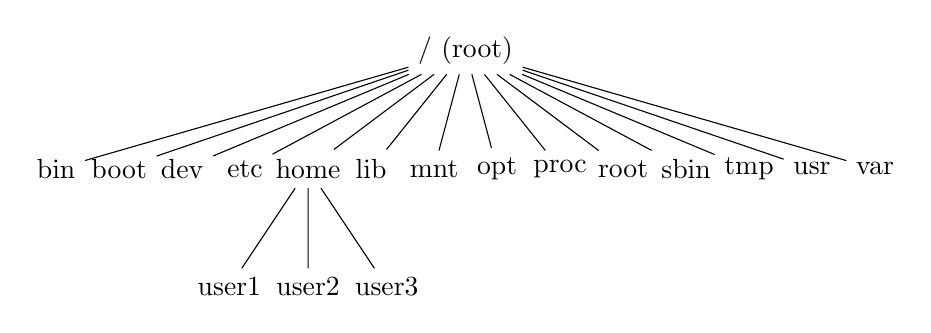
\begin{tikzpicture}[
      level 1/.style={sibling distance=8mm},
      level 2/.style={sibling distance=10mm}
    ]
    \node {/ (root) }
        child {
          node {bin}
        }
        child {
          node {boot}
        }
        child {
          node {dev}
        }
        child {
          node {etc}
        }
        child {
          node {home}
          child {
            node {user1}
          }
          child {
            node {user2}
          }
          child {
            node {user3}
          }
        }
        child {
          node {lib}
        }
        child {
          node {mnt}
        }
        child {
          node {opt}
        }
        child {
          node {proc}
        }
        child {
          node {root}
        }
        child {
          node {sbin}
        }
        child {
          node {tmp}
        }
        child {
          node {usr}
        }
        child {
          node {var}
        }
      ;
  \end{tikzpicture}
\end{flushleft}
      

\end{itemize}
\end{frame}

\begin{frame}[t]
\frametitle{Pregled direktorija sustava (3)}
\begin{itemize}
  \item Sadržaj datoteka definiran je FHS standardom\\ (engl.
        \emph{Filesystem Hierarchy Standard})
  \begin{itemize}
    \item Struktura sustava ipak nije ista za sve Unix sustave
  \end{itemize}
  \item Definirani su direktoriji neposredno ispod korijenskog direktorija
        i neki njihovi poddirektoriji
  \item[] \texttt{/}
  \begin{itemize}
    \item Datotečni sustav organiziran je u hijerarhiju koja počinje od
          \texttt{/} (\emph{root})
  \end{itemize}
\end{itemize}
\end{frame}

\begin{frame}[t]
\frametitle{Pregled direktorija sustava (4)}
\begin{itemize}
  \item[] \texttt{/bin}
  \begin{itemize}
    \item Korisnički i administratorski alati bez obzira da li je sustav u
          jednokorisničkom ili višekorisničkom načinu rada
  \end{itemize}
  \item[] \texttt{/boot}
  \begin{itemize}
    \item Jezgra operacijskog sustava i sve potrebno kako bi se operacijski
          sustav mogao pokrenuti tijekom podizanja sustava
          (engl. \emph{booting})
  \end{itemize}
\end{itemize}
\end{frame}

\begin{frame}[t]
\frametitle{Pregled direktorija sustava (5)}
\begin{itemize}
  \item \texttt{/dev}
  \begin{itemize}
    \item Direktorij s posebnim datotekama koje predstavljaju različite 
          uređaje 
  \end{itemize}
  \item \texttt{/etc}
  \begin{itemize}
    \item Konfiguracijske datoteke cijelog sustava 
  \end{itemize}
  \item \texttt{/lib} (\texttt{/lib64})
  \begin{itemize}
    \item Biblioteke nužne za rad sustava 
    \item Tu se nalaze moduli operacijskog sustava.
  \end{itemize}
\end{itemize}
\end{frame}

\begin{frame}[t]
\frametitle{Pregled direktorija sustava (6)}
\begin{itemize}
  \item \texttt{/lost+found}
  \begin{itemize}
    \item Datoteke vraćene nakon pada sustava
  \end{itemize}
  \item \texttt{/media}
  \begin{itemize}
    \item Direktorij unutar kojega se automatski dodaju pokretni
          uređaji/mediji kada se priključe na računalo, primjerice
          CD-ROM-ovi, USB diskovi, \ldots
  \end{itemize}
  \item \texttt{/mnt}
  \begin{itemize}
    \item Direktorij na koji (ili unutar kojega) korisnik ručno dodaje
          pokretne uređaje/medije
  \end{itemize}
\end{itemize}
\end{frame}

\begin{frame}[t]
\frametitle{Pregled direktorija sustava (7)}
\begin{itemize}
  \item \texttt{/opt}
  \begin{itemize}
    \item Instalacije programa koji nisu dio standardnog sustava
    \item Programi i pripadajuće datoteke se nalaze unutar jednog 
          direktorija.
  \end{itemize}
  \item \texttt{/proc}
  \begin{itemize}
    \item Sadrži virtualne datoteke koje se mijenjaju ovisno o stanju 
          sustava
    \item Pisanje u neku od datoteka može promijeniti ponašanje sustava.
  \end{itemize}
\end{itemize}
\end{frame}


\begin{frame}[t]
\frametitle{Pregled direktorija sustava (8)}
\begin{itemize}
  \item \texttt{/sbin}
  \begin{itemize}
    \item Sistemski programi koje administrator sustava treba imati na 
          raspolaganju za podizanje sustava.
  \end{itemize}
  \item \texttt{/tmp}
  \begin{itemize}
    \item Direktorij za privremenu pohranu datoteka
    \item U njega mogu pisati svi korisnici i najčešće ga koriste 
          aplikacije za spremanje datoteka tijekom rada
  \end{itemize}
\end{itemize}
\end{frame}

\begin{frame}[t]
\frametitle{Pregled direktorija sustava (9)}
\begin{itemize}
  \item \texttt{/var}
  \begin{itemize}
    \item Datoteke koje se često mijenjaju poput logova i pošte
  \end{itemize}
  \item \texttt{/srv}
  \begin{itemize}
    \item Direktoriji s podacima koji se nude korisnicima preko servisa
    \item Primjer su web stranice preko HTTP protokola i binarne datoteke
          preko FTP protokola.
  \end{itemize}
\end{itemize}
\end{frame}

\begin{frame}[t]
\frametitle{Pregled direktorija sustava (10)}
\begin{itemize}
  \item \texttt{/home}
  \begin{itemize}
    \item Matični direktoriji korisnika smješteni su unutar ovog
          direktorija
    \item Svaki korisnik posjeduje svoj direktorij gdje se nalaze osobne 
          datoteke korisnika
    \item Postavke aplikacija za pojedinog korisnika nalaze se u njegovom 
          matičnom direktoriju, u skrivenim datotekama.
  \end{itemize}
  \item \texttt{/root}
  \begin{itemize}
    \item Matični direktorij \emph{root} korisnika 
  \end{itemize}
\end{itemize}
\end{frame}

\section{Struktura \texttt{usr} direktorija}
\begin{frame}[t]
\frametitle{Struktura \texttt{usr} direktorija (1)}
\begin{itemize}
  \item \texttt{/usr}
  \begin{itemize}
    \item Sadrži vlastitu strukturu
    \item Za razliku od \texttt{/sbin} i \texttt{/bin} direktorija, koji 
          sadržavaju programe za osnovnu funkcionalnost sustava, ovdje su 
          programi za normalan rad sa sustavom
    \item[]
    \item[] \texttt{/usr/bin}
    \begin{itemize}
      \item Korisnički programi za opći rad sa sustavom
    \end{itemize}
    \item[] \texttt{/usr/sbin}
    \begin{itemize}
      \item Programi za cjelokupnu administraciju sustava
    \end{itemize}
  \end{itemize}
\end{itemize}
\end{frame}

\begin{frame}[t]
\frametitle{Struktura \texttt{usr} direktorija (2)}
\begin{itemize}
  \item Raspodjela \texttt{/usr},\texttt{/bin} i \texttt{/sbin} nije uvijek
        precizno definirana i ovisi o implementaciji Unix sustava
  \item[]
  \item[] \texttt{/usr/local}
  \begin{itemize}
    \item Instalacije programa na lokalnom sustavu
    \item Sadrži poddirektorije \texttt{/usr/local/bin} i 
          \texttt{/usr/local/sbin}
    \item U \texttt{/usr/local} nalazili su se programi specifični za 
          pojedinog korisnika, dok su se u ostalim direktorijima nalazili
          programi za sve korisnike
  \end{itemize}
\end{itemize}
\end{frame}

\section{Pregled zauzeća diskovnog prostora}
\begin{frame}[t]
\frametitle{Naredba \texttt{df}}
\begin{itemize}
  \item Naredba \texttt{df} ispisuje zauzeće po particijama
  \begin{itemize}
    \item Najčešće se koristi s opcijom \texttt{-h}
  \end{itemize}
  \item Zadatak
  \begin{itemize}
    \item Koliko je zauzeće po particijama na sustavu?
  \end{itemize}
\end{itemize}
\end{frame}

\section{Pregled zauzeća direktorija}
\begin{frame}[t]
\frametitle{Naredba \texttt{du}}
\begin{itemize}
  \item Zauzeće prostora po direktorijima se provjerava naredbom
        \texttt{du}
  \item Moguće je ispisivanje zauzeća po poddirektorijima do određene
        razine
  \item Zadatak
  \begin{itemize}
    \item Ispišite zauzeće matičnog direktorija do prve razine u čitljivom
          (engl. \emph{human readable}) obliku, s ispisivanjem ukupnog 
          zauzeća na kraju ispisa
  \end{itemize}
\end{itemize}
\end{frame}

\end{document}
